\section{Introduction to single cell transcriptomics}

Cells are the fundamental units of life, forming the basis of all living organisms.
One of the major goals of biology is to understand cellular systems and the processes occurring within cells.
Since the discovery of the DNA structure in 1953
and the development of the conceptual framework for genetic information transfer (\cite{Watson1953}),
scientists have made significant efforts to sequence the genomes of various organisms.
This led to the development of the first sequencing methods, such as Sanger sequencing in 1975 (\cite{Sanger1977}),
which laid the foundation for next-generation sequencing (NGS) technologies in use today,
such as the widely used Illumina platform (\cite{Heather2016}).
Current sequencing methods allow us to obtain the complete genetic sequence of any organism.
However, the genome alone cannot explain the full diversity of cells in multicellular organisms,
as all cells share the same genome but exhibit significant variation in shape, size, and function.

RNA sequencing (RNAseq), on the other hand, enables the measurement of gene expression within cells,
providing valuable insights into cellular processes.
RNAseq methods largely follow DNA sequencing protocols,
with the addition of a step where complementary DNA (cDNA) is synthesized from RNA (\cite{Heumos2023}).
The first RNAseq methods were developed for bulk sequencing, where RNA from entire cell populations is sequenced,
providing an average gene expression profile across the population.
Although bulk RNAseq has provided valuable insights into the dynamics of cellular processes
(such as changes in disease states in response to therapeutics, detection of gene isoforms, gene fusions,
and various other properties of target cells (\cite{Heumos2023})),
this approach masks non-dominant processes and cell-to-cell variability through averaging.
This limitation was addressed by the introduction of single-cell RNA sequencing (scRNAseq) methods,
which allow for the generation of transcriptomic profiles from individual cells,
providing high-resolution insights into cellular systems.

Current scRNAseq methods enable the generation of transcriptomic profiles from thousands of cells
at unprecedented resolution in a single experiment.
These data can be used for constructing cellular atlases (\cite{Rozenblatt2017}),
understanding disease mechanisms (\cite{Zhang2024}),
exploring cell differentiation and developmental processes (\cite{Skinner2024}), among many other applications.

\section{scRNAseq data generation and analysis}

\subsection{Overview of scRNAseq protocols}

The generation of scRNA-seq data is a complex, multi-step process that varies across different protocols.
These protocols can be grouped based on several criteria, such as the type of RNA capture
(e.g., 3' end, 5' end, or full-length) or the method of cell isolation
(e.g., droplet-based methods such as inDrops (\cite{Klein2015}), Drop-seq (\cite{Macosko2015}),
and Chromium by 10X Genomics (\cite{Zheng2017}),
or plate-based methods such as CEL-Seq2 (\cite{Hashimshony2016}) and Smart-seq2 (\cite{Picelli2013})).

In this project, datasets generated using droplet-based 3' end sequencing methods were analyzed.
Therefore, these methods will be the focus of the following literature review.

\paragraph{3' End Sequencing and Polyadenylation}

3' end sequencing captures RNA molecules using primers complementary to poly(A) tails.
Polyadenylation at the 3' end is a post-transcriptional modification
in which non-templated adenosines are added to the 3' end of mRNA molecules.
Although the poly(A) tail is present in almost all mRNAs,
its length varies and can influence mRNA fate, stability, and translation efficiency (\cite{Brouze2022}).

3' end sequencing protocols exploit this feature to selectively capture RNA molecules,
enabling high-throughput and cost-effective sequencing.
However, some RNA molecules lack poly(A) tails and are therefore not captured by these methods,
such as replication-dependent histone mRNAs (\cite{Brouze2022}).

\paragraph{Common Steps in scRNA-seq Protocols}

Despite differences between scRNA-seq protocols, they share key steps:
single-cell isolation, library preparation, and sequencing (\cite{Andrews2018}).
In droplet-based methods, single cells are encapsulated in individual droplets containing hydrogel-attached barcoding primers
and a lysis mix (an example of a droplet generation device is shown in Figure \ref{fig:inDropsDevice}).
Primers used in these protocols typically share a common structure, including:

\begin{figure}
  \centering
  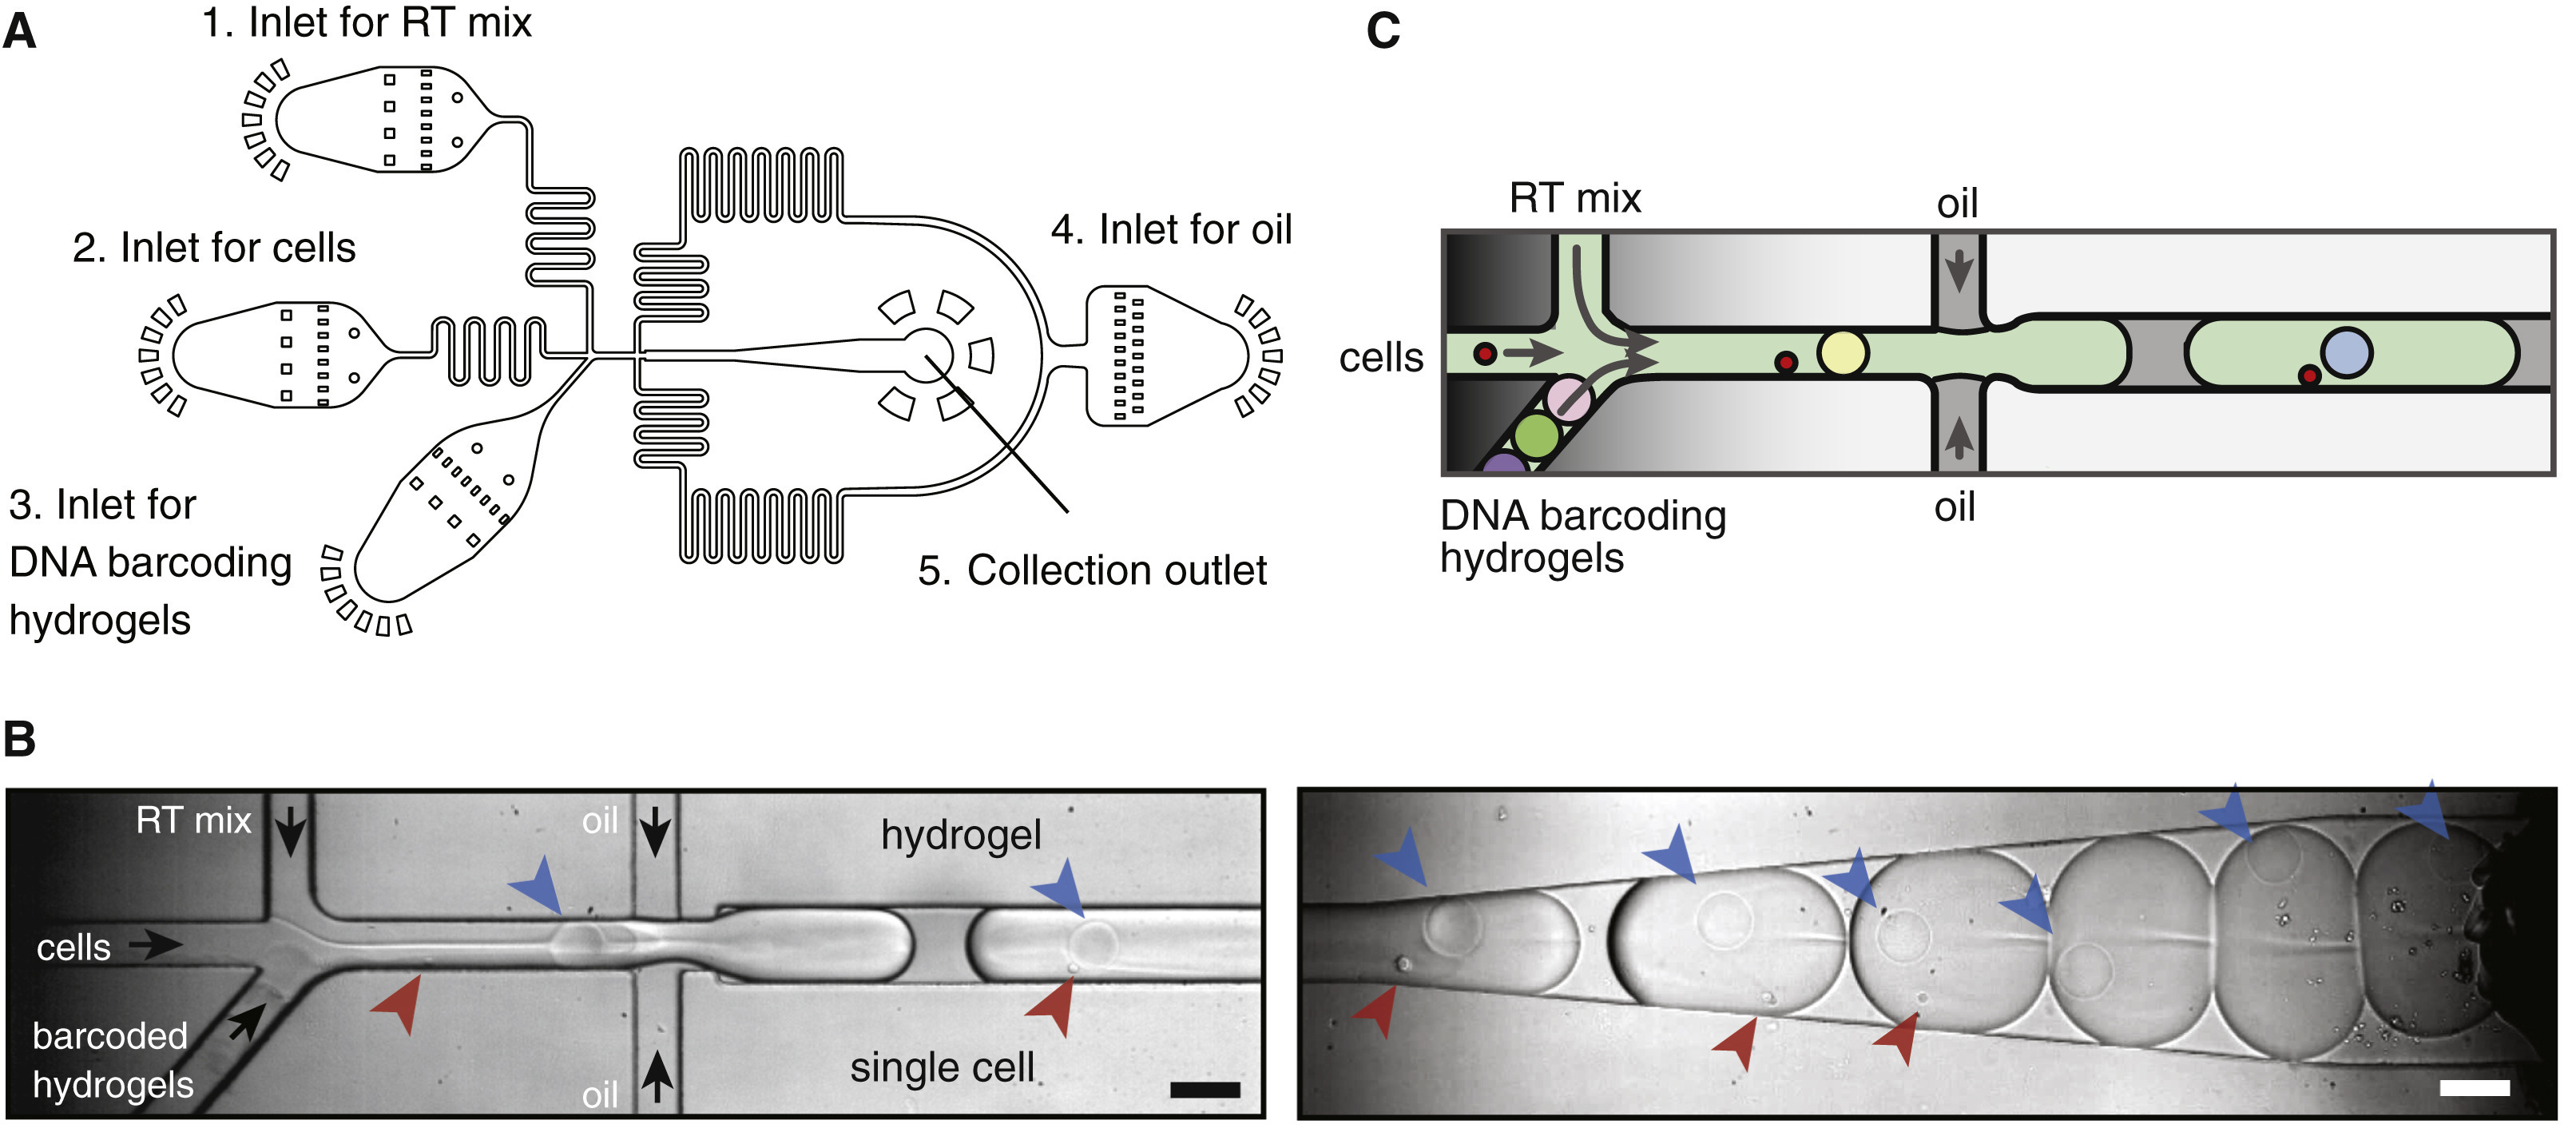
\includegraphics[width=\linewidth]{images/indropsDevice.jpg}
  \caption{An example of microfluidics device for droplet generation (inDrops).
  A) Schematic view of the device.
  B) Snapshots of droplet generation and colection.
  C) Scheme of droplet generation.
  Figure taken from \textcite{Klein2015}.}
  \label{fig:inDropsDevice}
\end{figure}

\begin{itemize}
  \item \textbf{Cell barcodes:} Unique sequences that identify the cell from which a particular read originates (since all droplets are pooled and sequenced together).
  \item \textbf{Unique molecular identifiers (UMIs):} Short sequences used to quantify the original number of RNA molecules, helping to eliminate amplification bias.
  \item \textbf{PCR handles:} Sequences that facilitate amplification.
  \item \textbf{Poly-T sequences}: In 3' end sequencing methods are used to selectively capture polyadenylated RNAs (\cite{Zhang2019}).
\end{itemize}
An example of primer design is shown in Figure \ref{fig:inDropsPrimer}.
Once cells are encapsulated in droplets, lysis occurs, releasing RNA, which is then captured by the primers.
A schematic overview of library preparation is provided in Figure \ref{fig:inDropsPipeline}.

\begin{figure}
  \centering
  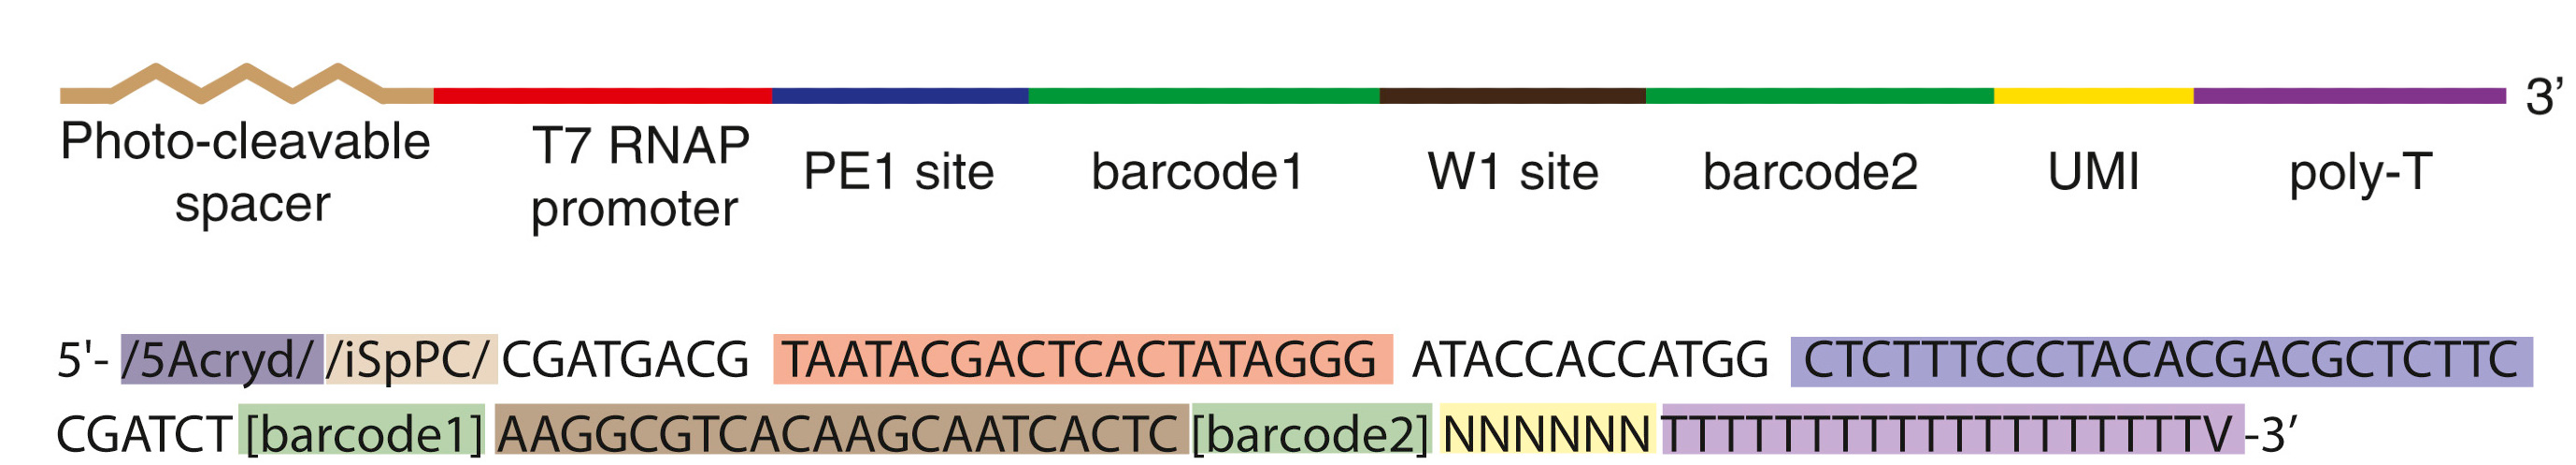
\includegraphics[width=\linewidth]{images/primer.png}
  \caption{Example of primer design (inDrops).
  The image above shows schematic view, while below is given example with sequences.
  The structure of primers varies between the protocols, the main parts (UMI site, barcodes, poly-T's)
  are found in most of them.
  Here also present are promoter region for RNA polymerase (red), sequencing primer (blue), synthesis adaptor (dark brown).
  Figure taken from \textcite{Klein2015}.}
  \label{fig:inDropsPrimer}
\end{figure}

\begin{figure}
  \centering
  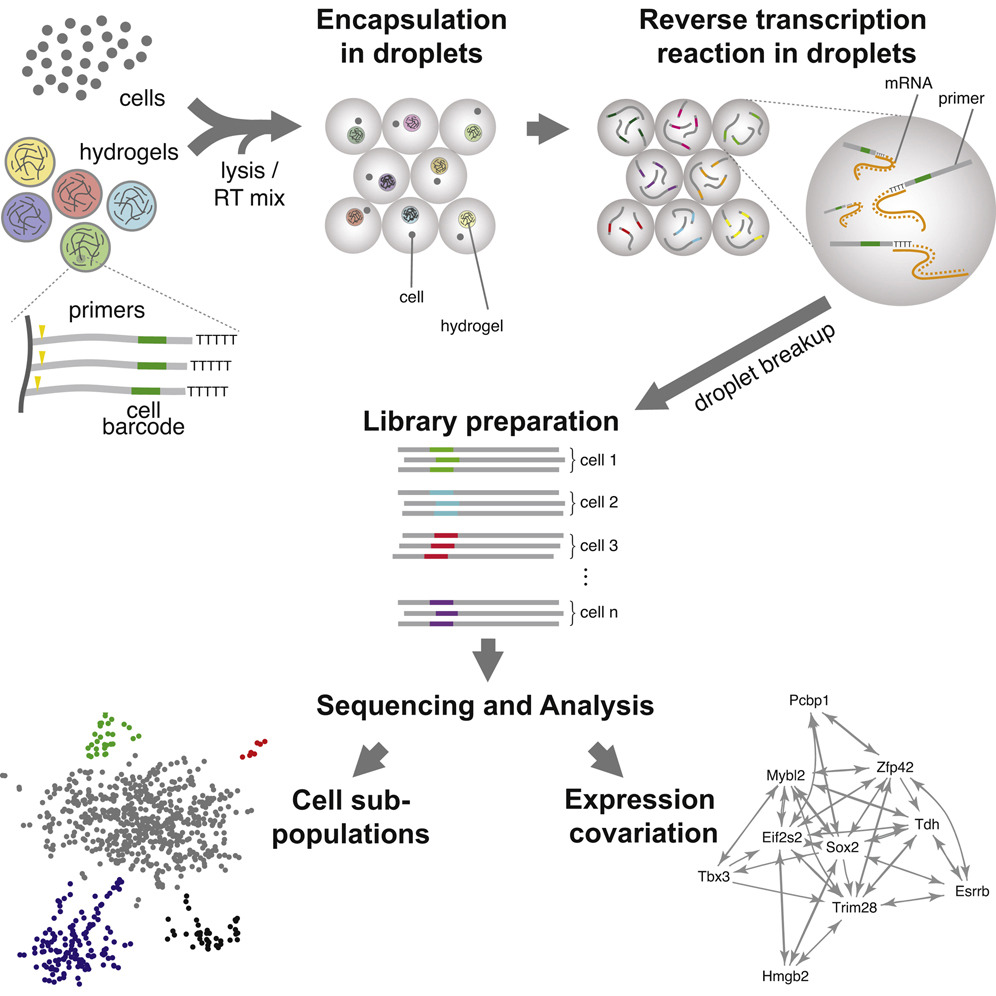
\includegraphics[width=\linewidth]{images/scAnalysisPipeline.jpg}
  \caption{The schematic presentation of droplet-based scRNAseq
  particularly inDrops, however main steps are shared between most of the droplet based protocols.
  Figure taken from \textcite{Klein2015}.}
  \label{fig:inDropsPipeline}
\end{figure}

Depending on the method, reverse transcription may occur within the droplets
(as in inDrops and 10X Genomics) or in bulk (as in Drop-seq).
Subsequent steps typically include RNA fragmentation, PCR amplification, and next-generation sequencing (NGS).	


\subsection{scRNAseq data analysis}

\paragraph{Raw data processing}

The output from NGS machines is typically converted to FASTQ files, containing recorded sequences,
as well as (depending on method) barcode and UMI sequences, and quality scores.
The subsequent processing steps include quality control of FASTQ file (based on quality scores),
filtering duplicate reads (using UMIs), mapping reads to the genome sequence, assigning the reads to the genes,
and finally, counting gene expression per cell (barcode) (\cite{Heumos2023}) (see figure \ref{fig:rawData}).
Usually, all these steps are performed with a single piece of dedicated software,
such as STARsolo (\cite{Kaminow2021}), CellRanger (\cite{Zheng2017}) or other.
It should be noted, that there are variations in the pipeline described above,
depending on many experiment-related (e.g., whether the genome sequence or transcriptone of the study organism is known),
or method-related (e.g., whether UMIs are used in the protocol) factors.
The typical result of such processing is cell-gene matrix (i.e., a matrix where rows represent cells,
columns represent genes, and each entry indicates the number of captured RNAs for a given gene in a specific cell).

\begin{figure}
  \centering
  
\includegraphics[width=\linewidth]{images/rawdata.png}
  \caption{Inputs and outputs of mapping software.}
  \label{fig:rawData}
\end{figure}

\paragraph{Cell-gene matrix processing}

The next steps in the analysis of the scRNAseq data involves following steps:

\begin{itemize}
  \item \textbf{Quality control}
The quality of indidual cells (represented as all reads harboring a unique barcode)
can be evaluated based on several factors, such as mitochondrial gene content
(apoptotic cells tend to have a higher proportion of mitochondrial transcripts (\cite{Heumos2023})) or
total number of captured genes (very low numbers can be produced by ambient RNA entering empty droplets).
In some cases, two cells can end up in one droplet,
resulting in count matrix row corresponding to genes from  both cells.
Such matrix entries (doublets) can be filtered by using specialized software
such as Scrublet (\cite{Wolock2019}) or scDblFinder (\cite{Germain2022}).
Another source of noise in scRNAseq data is ambient RNA,
which consists of RNA that escapes individual droplets and spreads into the medium or other droplets,
leading to background noise.
Even though the amount of such RNA is not high (in good quality datasets it can be around 2\% (\cite{Young2020})),
removing these RNAs from the count matrix can improve data quality.
This can be achieved by identifying the background noise profile from empty droplets and
adjusting the count matrix accordingly.
There are dedicated softwares,
such as SoupX (\cite{Young2020}), decontX (\cite{Yang2020}), CellBender (\cite{Fleming2023}) and others.
  \item \textbf{Normalization}
The next step in preprocessing pipeline is normalization.
The goal of normalization is to transform the data so that the variation in gene expression levels is comparable,
making subsequent analysis more efficient (\cite{Ahlmann2023}).
Normalization can also help eliminate biases,
such as differences in sequencing depth when combining data from multiple samples (\cite{Lingen2024}).
There are numerous normalization methods, based on different approaches
(e.g., delta-method-based, residual-based, latent gene expression-based, count-based (\cite{Ahlmann2023})).
Thus, selecting a normalization method should be done carefully, depending on the experimental design.
General recommendations for normalization suggest comparing several methods,
and if the results are similar, opting for the simpler method (\cite{Lingen2024}).
Sophisticated methods do not necessarily show better results, and a recent benchmarking study by \textcite{Ahlmann2023}
has shown that simpler method (particularly the logarithm normalization,
where each element $y$ of count matrix is transformed by formula $y_{trnasformed} = log(y+1)$)
performs as well or better than more advanced methods.
\item \textbf{Filtering genes}
Once the data is normalized and cleaned, one can filter out non-informative genes.
Initially, count matrices contain all the genes that are present in the transcriptome.
However, not all of them are expressed in the sequenced data, or are expressed in negligible numbers (\cite{Heumos2023}).
Therefore, it is common practice to filter such genes (e.g., genes that are expressed in less than three cells).
Moreover, some genes might be expressed in all the cells more or less evenly (housekeeping genes),
which do not provide useful information that could be usefull in, for instance, grouping cells or determining cell types.
Therefore, in many applications, it is beneficial to leave only those genes, that are highly variable between cells.
In such way, the dimensionality of the count matrix is greatly reduced without loosing significant information.
Additionally, genes that are outside the scope of the specific study can also be filtered out.
\item \textbf{Dimensionality reduction}
Even after filtering and selecting only highly variable genes, several thousand genes usually remain.
It is not feasible to visualize (and hard to interpret in general) data of such high dimentionality, therefore,
dimensionality reduction is essential step of subsequent analysis.
The idea of dimentionality reduction is simple:
to reduce the dimentions of the data loosing as little information as possible.
There are a number of dimensionality reduction methods based on different mathematical concepts,
but the most widely used today include
t-SNE (\cite{Hinton2002}), UMAP (\cite{McInnes2018}) and principal component analysis (PCA).
Although the use of these algorithms are supported by some benchmarking studies
(in the study of \textcite{Xiang2021}, t-SNE was showed best performance, while UMAP showed the highest stability),
other benchmarking studies report different findings.
The study of \textcite{Koch2021} suggested that such overlooked methods as
latent Dirichlet alloacation (LDA) and PHATE are among the best performing
(metrics for comparison included clustering accuracy, structure preservation, efficiency and others).
Meanwhile \textcite{Sun2019} provided guidelines for choosing dimensionality reduction method
depending on downstream analysis tasks, and in their results UMAP and tSNE were not on the top choices.
Thus, while UMAP remains the gold standard method in the field (usually preceded by PCA for initial dimensionality reduction),
it is worth considering alternative methods as well.
\item \textbf{Clustering and other analyses}
One of the most common tasks of scRNAseq data analysis is to identify and classify cell populations (\cite{Andrews2018}).
This task requires to assign cells to different groups (clusters),
such that cells in the same clusters are similar and distinct from cells in other clusters.
There is a great variety of clustering algorithms available,
including k-means, hierarchical and consensus clustering (\cite{Peng2020}).
Benchmarking studies suggest that "no individual scRNA-seq clustering algorithm can capture true clusters and achieve
optimal performance in all situations" (\cite{Peng2020}).

Clustering is usually followed by cell annotation (i.e., assigning cell type to the identified clusters),
which is done by finding cell type specific markers
or using automatic (machine learning) tools such as CellTypist (\cite{Dom2022}).
The subsequent steps in the analysis depend on the focus of the particular study and can include
differential gene expression (dge) analysis,
investigation of the dynamics of cellular systems (RNA velocity, pseudotime),
inferring gene regulatory networks (GRNs), and more.
\end{itemize}

The described analysis pipeline enables insights into multicellular systems.
It is evident that all downstream analyses are directly influenced by the initial steps of raw data processing,
with mapping being particularly crucial in the context of this project.
While mapping algorithms and tools differ, they all rely on the genome and its annotation (also refered as 'transcriptomic reference'),
which directly impact their results.
In the next section, I will further expand on this topic.

\section{Genome annotation}

The genome annotation process typically refers to the identification and mapping of genes within a given genome sequence (\cite{Guigo2023}).
While the definition itself is straightforward, the process is highly complex.
This is evident from the fact that, even more than 20 years after the first human genome assembly,
human genome annotations are continuously updated with new transcripts and are expected to evolve further (\cite{Mudge2024}).
Figure \ref{fig:gencode} illustrates the changes in GENCODE annotation over time.

It is important to note that many medical and scientific research efforts rely on an accurate human gene list.
Examples include genome-wide association studies (GWAS), which attempt to link genomic variants to nearby genes;
RNA-seq analysis; and exome sequencing projects that use capture kits targeting most known exons (\cite{Pertea2018}).

Currently, the two most widely used genome annotations are GENCODE (\cite{Mudge2024}) and RefSeq (\cite{OLeary2015}) (maintained by NCBI).
Despite their status as mature genome references, they report different numbers of genes.
For instance, RefSeq includes 20,078 protein-coding genes (\cite{ncbi}), whereas GENCODE contains 19,868 (\cite{ensembl}).
This discrepancy highlights the ongoing challenge of accurately annotating genomes.

\paragraph{Genome annotation process}

RNA sequencing (RNA-seq) is the primary tool used in genome annotation.
Full-length RNA sequencing allows for the capture of RNA molecules, which, when aligned to a reference genome,
help construct the genome annotation of a given species (\cite{Salzberg2019}).
However, RNA-seq has limitations, the most significant being its inability to capture all RNA molecules.
This poses particular challenges for detecting rare transcripts, which may either be treated as noise or not captured at all (\cite{Salzberg2019}).
Therefore, bioinformatics tools are necessary to complement RNA-seq data (\cite{Guigo2023}),
and most modern genome annotation pipelines integrate computational methods alongside sequencing data.

Computational genome annotation methods can be broadly categorized into two types:
comparative annotation, which leverages the fact that protein-coding sequences tend to be more evolutionarily conserved,
and \textit{ab initio} annotation, which uses known sequence biases to predict genes (\cite{Guigo2023}).
Despite significant advancements, genome annotation remains imperfect.

While the number of protein-coding genes is reaching a consensus — major databases report around 19,000 to 20,000 protein-coding genes — 
the number of non-coding genes is expected to increase in the future (\cite{Amaral2023}).
This is largely due to the structured nature of protein-coding genes (e.g., open reading frames, codon biases that skew nucleotide distributions),
which makes them easier to detect using computational tools (\cite{Guigo2023}).
Additionally, protein-coding genes have historically received greater attention because of their direct links to phenotype,
leading to more experimental validation.

\paragraph{Current challenges in human genome annotation}

Despite extensive efforts, a fully comprehensive human genome annotation has not yet been achieved.
Several factors contribute to this challenge.

Firstly, the complexity of the human genome itself presents significant obstacles.
Compared to the total genome length, the number of genes is relatively low, and their sequences are interrupted by introns (\cite{Salzberg2019}).
Additionally, bulk RNA sequencing often has relatively low sequencing depth,
making it difficult to detect rare transcripts or those expressed in a cell-type-specific manner (\cite{Guigo2023}).

In principle, full-length single-cell RNA sequencing (scRNA-seq) could help overcome some of these limitations.
However, it still has inherent biases introduced during library preparation, including those related to RNA processing status,
post-transcriptional modifications, transcript length, cellular localization, and structural features (\cite{Guigo2023}).
Short-read scRNA-seq typically provides higher throughput (\cite{Heumos2023}), enabling the detection of rare transcripts.
However, it does not capture full transcript structures, limiting its utility to supporting evidence,
such as validating computationally predicted genes or indicating transcriptional activity at specific genomic locations.

Beyond technical limitations, there are ontological challenges, such as defining what constitutes a gene.
While genes are often regarded as well-defined, discrete entities, the reality is more complex.
Coding and non-coding transcripts frequently overlap in intricate arrangements with unclear boundaries,
suggesting that transcripts may not be discrete, countable units but instead form a transcriptional continuum (\cite{Salzberg2019}).
Additionally, the classification systems used in genome annotations may be partially artificial.
For example, some pseudogenes, generally considered non-functional copies of functional genes,
are transcribed and may have biological functions (\cite{Pei2012}).
Similarly, the distinction between protein-coding and non-coding genes is debated, as many protein-coding loci generate both coding
and non-coding transcripts, and numerous long non-coding RNAs (lncRNAs) contain potentially coding  open reading frames (ORFs) (\cite{Salzberg2019}).

\paragraph{Future perspectives of annotating genomes}

The size of eukaryotic genomes necessitates the use of automated methods for genome annotation.
The accuracy of such methods depends directly on RNA capture technologies.
If highly accurate and sensitive methods are developed, high-quality genome annotations can be expected (\cite{Salzberg2019}).
However, at present, manual curation of human genome annotations remains essential due to the imperfections of both sequencing technologies
and computational tools.
Given the critical role of accurate gene annotation in both medical and scientific applications,
continued improvements in annotation methods remain a priority.

\begin{figure}
  \centering
  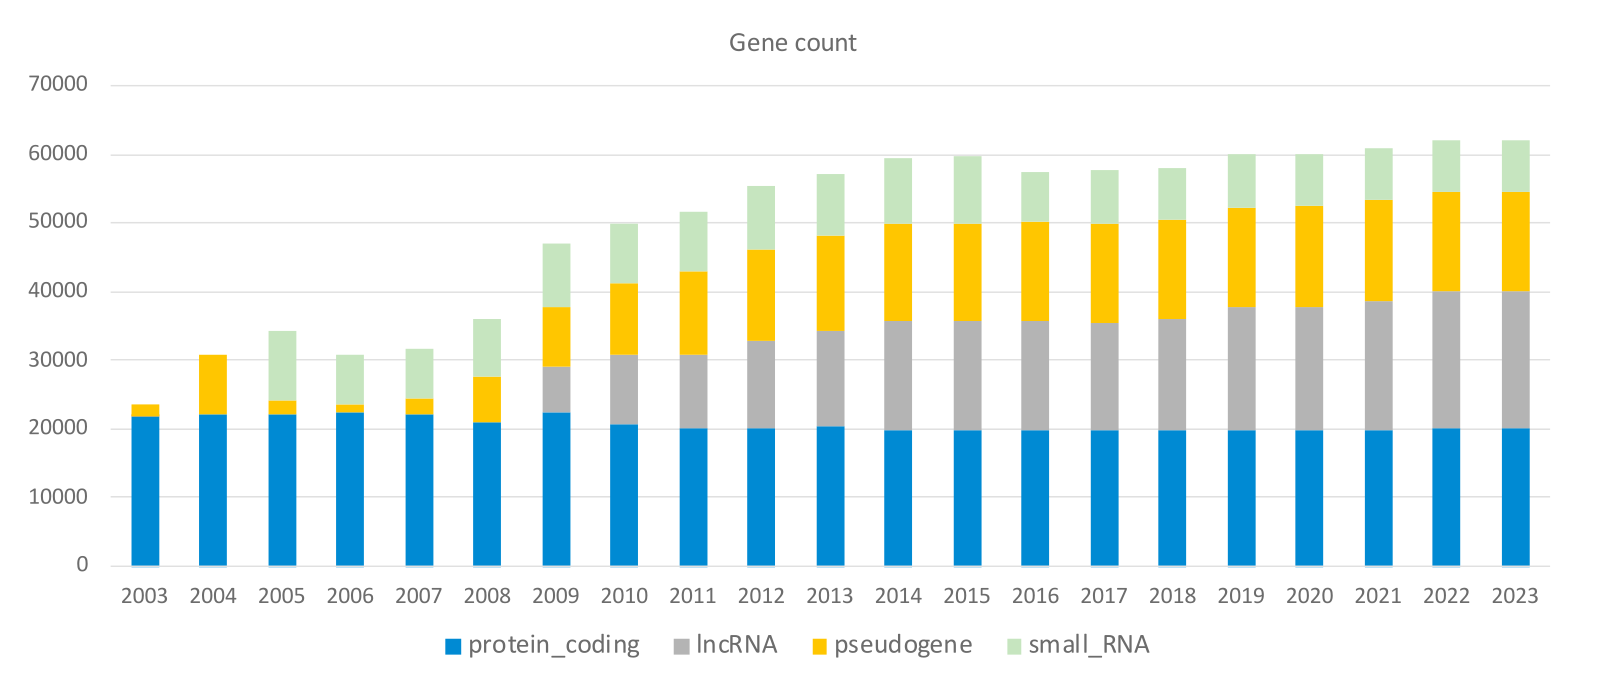
\includegraphics[width=\linewidth]{images/gencode.png}
  \caption{Number of different genes in the gencode annotation during time. Figure taken from paper by \textcite{Guigo2023}}
  \label{fig:gencode}
\end{figure}

\section{Transcriptomic references for scRNAseq}

Having a well-annotated genome does not solve all the challenges encountered during the mapping step.
In simple terms, mapping algorithms determine the genomic location to which a sequence aligns,
and if an annotated gene is present at that location, the read is assigned to that gene.
However, there are cases where assigning a read to a gene is not straightforward,
such as when a read maps to multiple locations or to a unique location where overlapping genes are annotated.

\paragraph{Multimappers}
There are two possible reasons for reads assigned to multiple genes: either they are mapped to multiple genome locations,
or they are mapped to the genomic location containing overlapping features (genes).
Such reads (commonly referred to as multimappers) are typically excluded from analysis (\cite{Paz2024}).
However, as demonstrated by (\textcite{Paz2024}), this approach can introduce biases that affect downstream analyses.
Currently, various methods exist to handle such cases (\cite{Francoeur2020}),
yet no entirely satisfactory solution has been established (\cite{Paz2024}).

The aforementioned methods primarily rely on computational strategies to resolve multimappers,
but the issue can also be approached from a transcriptomic reference perspective.
For example, in the case of CellRanger (the mapping software from 10x Genomics)
the GENCODE reference is filtered based on gene types (e.g., retaining protein-coding genes while filtering out pseudogenes) (\cite{10xRef}).
While this filtering improves the number of reads included in downstream analyses, there is still room for improvement.

\textcite{Pool2023} proposed three key steps to enhance transcriptomic references:
\begin{enumerate}
  \item Including reads mapped to intronic sequences in the analysis.
  \item Extending the 3' ends of certain genes.
  \item Resolving overlaps between specific genes.
\end{enumerate}
The first suggestion is not new in scRNA-seq research.
Concepts such as RNA velocity, which rely on the ratio of spliced to unspliced RNA (\cite{Manno2018}),
demonstrate that including intronic reads can provide valuable information.
Moreover, most mapping tools (e.g., STARsolo, CellRanger) offer options to align reads either to exonic regions only or to entire genes.
The second suggestion is based on the observation that scRNA-seq data often exhibits peaks of reads just beyond the 3' ends of genes.
While the exact biological reasons remain unclear — possibly due to imprecise annotations —
it is reasonable to associate these reads with the nearest genes.
The third suggestion addresses gene overlaps.
Reads originating from overlapping regions are often unassigned to any gene,
yet in some cases, they are more likely to come from one gene rather than another.
Overlapping gene resolution seeks to correct this by modifying the transcriptomic reference, either by shortening or removing certain genes.

Although \textcite{Pool2023} proposed a tool to implement these strategies, it has limitations.
Some of its aspects remain debatable (e.g., threshold choices), others seem unnecessary
(such as handling exon-intron distinctions when most alignment tools already provide this option),
and the process still requires significant manual effort.
Thus, there is still a need for a more comprehensive tool for enhancing transcriptomic references — a need that will be addressed in this thesis.

\paragraph{Reads mapped to the intergenic regions}
Some reads map to the genome but not to any annotated gene.
While these could simply be noise in scRNA-seq data, there is also the possibility that they contain biologically relevant information.
As will be shown in the results section, scRNA-seq datasets indeed contain such reads, and they are not entirely noise.































\iffalse
\section{Key methods and technologies in scRNAseq}

\subsection{Key methods}

All scRNAseq protocols share these main three steps:
isolation of single cells, library preparation and sequencing (\cite{Andrews2018}).

\begin{itemize}
  \item \textbf{Isolation of single cells:} Cells are separated from each other
  and placed into different droplets (microfluidics approach)
  or into different wells (plate-based approach).
  \item \textbf{Library preparation:} The next generation sequencing (NGS) usually requires nanograms or more of DNA,
  and the RNA content in single cells is far from this amount (\cite{Wu2017}).
  Consequently, before sequencing, reverse transcription (RT) and amplification is needed.
  Additionally, usually cell barcode sequences and unique molecular identifiers are attahced to the transcripts (before amplification),
  which later allows one to identify cell of origin for each read and real number of counts.
  \item \textbf{Sequencing:} NGS methods are used for the scRNAseq sequencing.
  Afterwards, acquired data can be processed and analyzed using bioinformatical methods.
\end{itemize}

Even though these steps are common to all scRNAseq protocals,
the variations in details give variations in the results, each one having its own strengths and weaknesses.
In the next section I will overview most popular platforms for scRNAseq.

\subsection{Current scRNAseq Platforms}

As mentioned before, scRNAseq methods mainly can be grouped in two groups: droplet-based and plate-based.

Droplet-based methods (e.g. inDrops (\cite{Klein2015}), Drop-seq (\cite{Macosko2015}),
Chromium by 10X Genomics (\cite{Zheng2017}))
separate cells by placing them into different droplets, which contain hidrogel primers and lysis mix.
Primers usually share a common structure, including barcode sequenes, unique molecular identifiers (UMIs),
PCR handlers and poly-T sequences (\cite{Zhang2019}).
Cell barcodes are sequences used for determining the cell from which a particular read was sequenced
(during sequencing, the content from all droplets is mixed and sequenced at once).
UMIs are used to quantify real amount of RNA in cells
(after amplification, more than one copy of each captured RNA is present).
PCR handlers are used for the amplification, while poly-T sequences are used for capturing RNAs.
An example of primer design can be seen in figure \ref{fig:primer}.
Once cells are in the droplets, cell lysis takes place, RNAs escape the cells and are captured by the primers.
Depending on method,
reverse transcription either takes place directly in the droplets (inDrops, 10X) or in bulk.
The next steps usually include RNA fragmentation and PCR amplification, followed by NGS.

Droplet-based methods are high-throughput
(current microfluidic devices are able to generate thousands of above described droplets per second (\cite{Prakadan2017})),
cost-effective, but have low detection rates compared to other methods and
captures only 3' (or 5') ends of transcripts (\cite{Heumos2023}).
Capturing only 3' ends of transcripts might be not a problem when trying to identify cell populations,
however, it masks such processes as splicing variants, thus should be considered carefully when planning experiments.

Plate-based methods (e.g. CEL-Seq2 (\cite{Hashimshony2016}), Smart-seq2 (\cite{Picelli2013}))
separate cells by placing them into different microwells on a plate.
Before this, cells can be sorted using, for example, fluorescent-activated cell sorting (FACS) (\cite{Heumos2023}).
Similarly to droplets, microwells contain lysis buffers and RT mix,
followed by amplification and NGS (\cite{Hashimshony2016}).
Barcodes can be integrated into reverse transcription step similarly as in droplet case.

Overall, plate-based methods have lower throughput, might be more costly and labor-intensive,
but offers recovery of many genes per cell, allows prior sorting and
(for some protocols) it is possible to sequence full transcripts (\cite{Heumos2023}).

In the next sections, we will focus on the droplet-based approaches,
as all the data used in this thesis is generated by droplet-based methods.

\begin{figure}
  \centering
  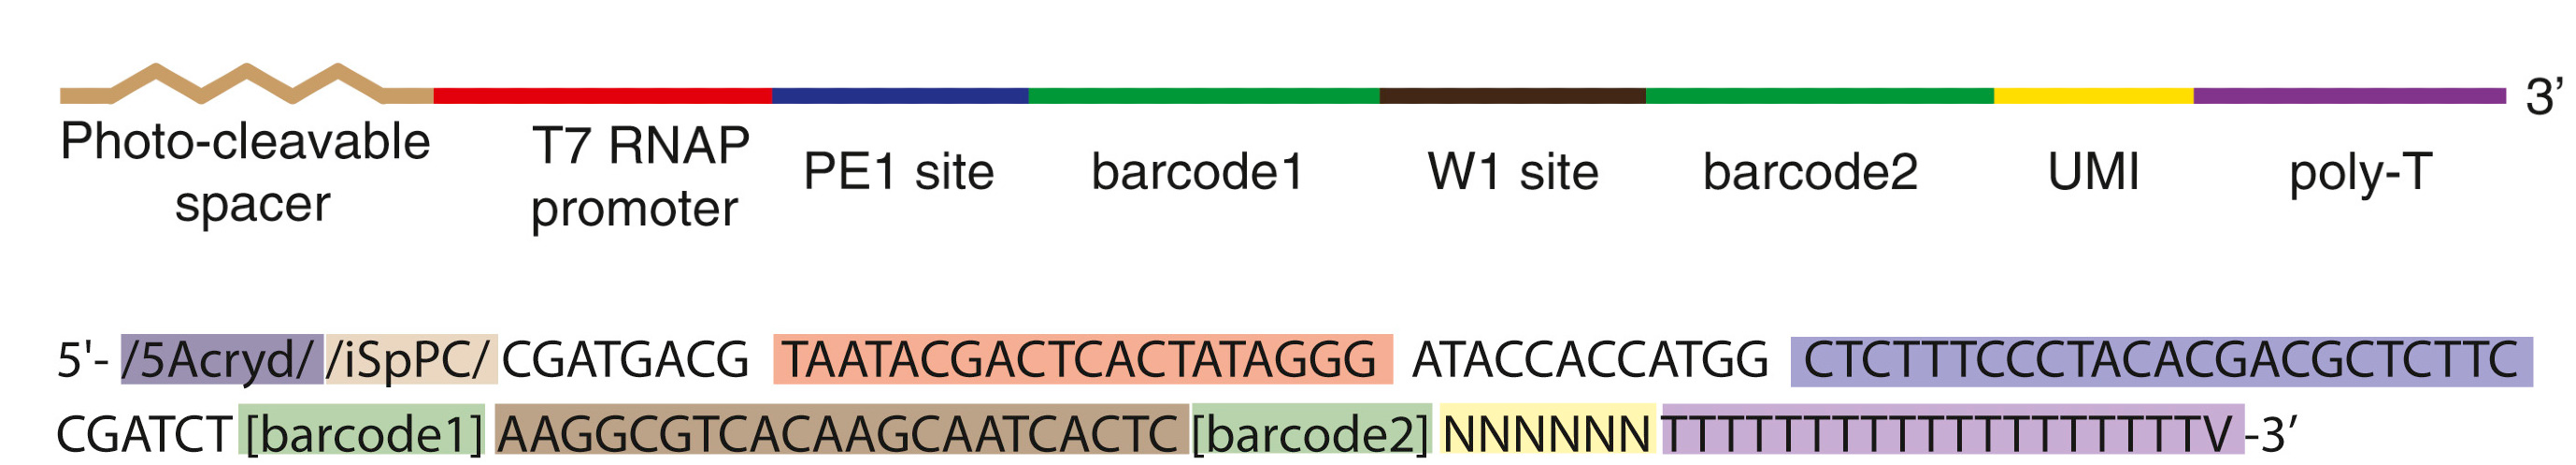
\includegraphics[width=\linewidth]{images/primer.png}
  \caption{Example of barcode (inDrops). The top image contains schematic view, while the bottom one shows example sequence.
           T7RNAP, PE1 and W1 sites here are used for primer assembly,
           while photo-cleavable spacer is used to release primers from the gel beads. Image taken from (\cite{Klein2015}).}
  \label{fig:primer}
\end{figure}

\section{Data quality and challenges in scRNAseq data}

The scRNAseq data offers high resolution insights in the cellular systems, however,
it comes with unique (and non-unique) challenges that need to be overcame to have clean, good-quality data.
In this section I will briefly overview noise sources and data scale challenges.

\subsection{Noise}

The noise in the scRNAseq data can have either biological or technical origin.
The biological noise is always present in the cellular systems due to the stochasticity of all biological processes (\cite{Vaz2017}).
While it is always in the data, more important is to eliminate technical noise.
Technical noise is the artefact of sequencing procedures.
The typical challenge in scRNAseq data is large number of dropout values (and consequently sparse data matrices).
I.e., if there is a zero entry in the cell-gene matrix, is not clear whether the gene was not expressed in the particular cell,
or was expressed but not captured.
This problem is particularly important if one is interested in rare transcripts.

Additionally, droplet-based methods introduce doublets and ambient RNA.
These two will be discussed in sections \ref{sec:preprocessingMatrices} and \ref{sec:imputation}.
In general, when the origin of noise is clear (as in doublets case), it is easier to make computational tools to eliminate it.
For dropout values, it is harder to say whether it is artefact or biological variability, hence eliminating such noise is very complex.

Finally, there are data quality challenges not specific to scRNAseq, such as batch effects.
While those are generally important, we will not focus on them in this review.

\subsection{Data scale and dimentionality}

Another challenge is data scale itself – typical scRNAseq datasets constains thousands of cells and tens of thousands of genes.
Such scales requires very efficiant analysis algorithms (some analysis tools are just too slow for using (\cite{McCalla2023})
and makes interpretability of data harder.
Many analysis pipelines uses dimensionality reduction to reduce the dimensions of the data (more on it in \ref{sec:dimReduction}).

\section{Computational tools and analytical approaches}

\subsection{Raw data processing}

The output of the typical scRNAseq experiment is FASTQ files, containing recorded sequences,
as well as (depending on method) barcode and UMI sequences, and quality scores.
The subsequent processing steps include quality control of FASTQ file (based on quality scores),
filtering dublicate reads (using UMIs), mapping reads to the genome sequence, assigning the reads to the genes,
and finally, counting gene expression per cell (barcode) (\cite{Heumos2023}) (see figure \ref{fig:rawData}).
Usually, all these steps are performed with a single piece of dedicated software,
such as STARsolo (\cite{Kaminow2021}), CellRanger (\cite{Zheng2017}) or others.
It should be noted, that there are variations in the pipeline described above,
depending on many experiment-related (e.g., whether the genome sequence or transcriptone of the study organism is known),
or method-related (e.g., whether UMIs are used in the protocol) factors.
The typical result of such processing is cell-gene matrix (i.e., a matrix where rows represent cells,
columns represent genes, and each entry indicates the number of captured RNAs for a given gene in a specific cell).

\begin{figure}
  \centering
  
\includegraphics[width=\linewidth]{images/rawdata.png}
  \caption{Pipeline of processing raw data.}
  \label{fig:rawData}
\end{figure}

\subsection{Preprocessing of count matrices}
\label{sec:preprocessingMatrices}

Preprocessing of count matrices usually involves these steps:
quality control, normalization and feature selection.

The quality of indidual cells can be evaluated based on several factors, such as mitochondrial gene content
(apoptotic cells tend to have a higher proportion of mitochondrial genes (\cite{Heumos2023})) or
total number of captured genes (very low numbers can be produced by empty droplets).
In some cases, two cells can end up in one droplet,
resulting in count matrix row corresponding to genes from  both cells.
Such matrix entries (doublets) can be filtered by using specialized software
such Scrublet (\cite{Wolock2019}) or scDblFinder (\cite{Germain2022}).
Another source of noise in scRNAseq data is ambient RNA,
which consists of RNA that escapes individual droplets and spreads into the medium or other droplets,
leading to background noise.
Even though the amount of such RNA is not high (in good quality datasets it can be around 2\% (\cite{Young2020})),
removing these RNAs from the count matrix can improve data quality.
This can be achieved by identifying the background noise profile from empty droplets and
adjusting the count matrix accordingly.
There are dedicated softwares,
such as SoupX (\cite{Young2020}), decontX (\cite{Yang2020}), CellBender (\cite{Fleming2023}) and others.

The next step in preprocessing pipeline is normalization.
The goal of normalization is to transform the data so that the variation in gene expression levels is comparable,
making subsequent analysis more efficient (\cite{Ahlmann2023}).
Normalization can also help eliminate biases,
such as differences in sequencing depth when combining data from multiple samples (\cite{Lingen2024}).
There are numerous normalization methods, based on different approaches
(e.g., delta-method-based, residual-based, latent gene expression-based, count-based (\cite{Ahlmann2023})).
Thus, selecting a normalization method should be done carefully, depending on the experimental design.
General recommendations for normalization suggest comparing several methods,
and if the results are similar, opting for the simpler method (\cite{Lingen2024}).
Sophisticated methods do not necessarily show better results, and a recent benchmarking study by \textcite{Ahlmann2023}
has shown that simpler method (particularly the logarithm normalization,
where each element $y$ of count matrix is transformed by formula $y_{trnasformed} = log(y+1)$)
performs as well or better than more advanced methods.

Once the data is normalized and cleaned, one can filter out non-informative genes.
Initially, count matrices contain all the genes that are present in the transcriptome.
However, not all of them are expressed in the sequenced data, or are expressed in negligable numbers (\cite{Heumos2023}).
Therefore, it is common practice to filter such genes (e.g., genes that are expressed in less than three cells).
Moreover, some genes might be expressed in all the cells more or less evenly (housekeeping genes),
which do not provide useful information that could be usefull in, for instance, grouping cells or determining cell types.
Therefore, in many applications, it is beneficial to leave only those genes, that are highly variable between cells.
In such way, the dimensionality of the count matrix is greatly reduced without loosing significant information.
Additionally, genes that are outside the scope of the specific study can also be filtered out.

\subsection{Dimensionality reduction}
\label{sec:dimReduction}

Even after filtering and selecting only highly variable genes, several thousand genes usually remain.
It is not feasible to visualize (and hard to interpret in general) data of such high dimentionality, therefore,
dimensionality reduction is essential step of subsequent analysis.
The idea of dimentionality reduction is simple:
to reduce the dimentions of the data loosing as little information as possible.
There are number dimensionality reduction methods based on different mathematical concepts,
but the most widely used today include
t-SNE (\cite{Hinton2002}), UMAP (\cite{McInnes2018}) and principal component analysis (PCA).
Although the use of these algorithms are supported by some benchmarking studies
(in the study of \textcite{Xiang2021}, t-SNE was showed best performance, while UMAP showed the highest stability),
other benchmarking studies report different findings.
The study of \textcite{Koch2021} suggested that such overlooked methods as
latent Dirichlet alloacation (LDA) and PHATE show best performance.
Meanwhile \textcite{Sun2019} provided guidelines for choosing dimensionality reduction method
depending on downstream analysis tasks, and in their results UMAP and tSNE were not on the top choices.
Thus, while UMAP and t-SNE remain the most popular methods in the field,
it is worth considering alternative methods as well.

\subsection{Clustering and other analyses}

One of the most common tasks of scRNAseq data analysis is to identify and classify cell populations (\cite{Andrews2018}).
This task requires to assign cells to different groups (clusters),
such that cells in the same clusters are similar and distinct from cells in other clusters.
There is a great variety of clustering algorithms available,
including k-means, hierarchical and consensus clustering (\cite{Peng2020}).
Benchmarking studies suggest that "no individual scRNA-seq clustering algorithm can capture true clusters and achieve
optimal performance in all situations" (\cite{Peng2020}).

Clustering is usually followed by cell typing (i.e., assigning cell type to the identified clusters),
which is done by finding cell type specific markers
or using automatic (machine learning) tools such as CellTypist (\cite{Dom2022}).
The subsequent steps in the analysis depend on the focus of the particular study and can include
analysis of the dynamics of cellular systems (RNA velocity, pseudotime),
inferring gene regulatory networks (GRNs), and more.

\section{Enhancing scRNAseq data}

Given the challenges associated with scRNAseq data, there have been attempts to improve the quality of such data.
In this section, I will provide an overview of two methods: data imputation and enhancing the transcriptomic reference.

\subsection{Data imputation}
\label{sec:imputation}

One of the challenges present in scRNAseq data is the large number of dropout values.
Dropout values refer to instances where gene expression is present in a cell but is missed in the scRNAseq data.
This problem can mask important relationships between genes and complicate downstream analysis (\cite{Wang2022}).
To impute dropout values, many tools have been suggested.
These methods can be divided into four categories:
model-based methods (bayNorm (\cite{Tang2019}), BISCUIT (\cite{Azizi2017}), SAVER (\cite{Huang2018}) etc.),
low-ranked matrix-based (ALRA (\cite{Linderman2022}), ENHANCE (\cite{Wagner2019}), scRMD (\cite{Chen2020}) etc.),
data smoothing methods (e.g. KNN-smoothing (\cite{Wagner2017}), MAGIC (\cite{Dijk2018}) etc.) and
deep learning methods (e.g. DCA (\cite{Eraslan2019}), DeepImpute (\cite{Arisdakessian2019}) etc.) (\cite{Wang2022}).

The study by \textcite{Dai2022} has shown that imputation methods are advantageous for recovering gene expression,
and among these methods, deep learning-based ones,
such as DCA, DeepImpute, scIGANs (\cite{Xu2020}) show the best performance.
However, it was also shown that imputation methods can introduce false positives.
In the study by \textcite{Andrews2019}, it was shown that data smoothing methods (e.g. MAGIC, KNN-smoothing)
generate most false positives among the different types of methods,
but other methods can generate relatively large number of false positives as well, depending on the dataset.
Data imputation does not necessarily improve downstream analysis
(e.g, it was shown that imputation doesn't improve inference of gene regulatory networks (\cite{McCalla2023})),
therefore one should carefully choose whether to impute data and which method to use.

\subsection{Enhancing transcriptomic reference}

One of the problems that scRNAseq is facing is the complexity of the genome.
The "raw" human transcriptomic reference (a file containing information about genes)
contains over 60000 genes (\cite{Frankish2022}).
Not all of these genes are expected to be captured by scRNAseq data
Thus, a simple approach to improving the transcriptomic reference is to filter out the genes
that are not expected to appear in scRNAseq data.
In this way, events where two genes overlap in the genome, but one is not expected to appear in the scRNAseq data,
are resolved, allowing alignment tools to more easily assign reads from these regions to the correct genes.
This approach is used in publicly available 10X transcriptomic references (\cite{Zheng2017}).
Even though it improves mapping performance, it does not address all the issues with the transcriptomc reference.

\textcite{Pool2023} has suggested three steps to enhance transcriptomic reference:
including reads mapped to intronic sequence to the analysis, extending 3' ends of some genes and
resolving overlaps between certain genes.
The first suggestion is not new in the field of scRNAseq.
There are concepts such as RNA velocity based on spliced an unspiced RNA ratio (\cite{Manno2018}),
showing that such including intronic reads in the analysis can provide valuable information.
Moreover, most mapping tools (e.g. STARsolo, CellRanger) contains options
to use either only exonic parts or full genes for read alignment.
The second suggestion is based on the observation,
that scRNAseq data often contains peaks of reads just after the 3' end of genes. 
While the exact biological reasons for this are unclear,
it makes sense to associate these reads with the genes they are closest to. 
The third suggestion focuses on resolving overlaps between genes.
Reads from such overlapping regions are often unassigned to any gene,
but in some cases, it is more likely that they originate from one gene rather than another.
Overlapping gene resolution aims to address this by deleting or shortening some genes in the transcriptomic reference.

Although \textcite{Pool2023} proposed the tool for such tasks, the tool is not without limitations:
some aspects of it are debatable (such as thresholds used), some seem unnecessarily
(e.g. handling exon and intron sequences when most alligning tools provide option for this),
and the process still requires a significant amount of manual work.
Thus, there remains a need for a more comprehensive tool for enhancing transcriptomic references,
which will be addressed in this thesis.

Another aspect, that should be taken into account, is that not all genes are known and annotated, even for such well-studied species as human.
Several tools were developed to predict de novo genes, such as AUGUSTUS (\cite{Stanke2008}), geneid (\cite{Blanco2007}), Gescan (\cite{Burge1997}),
SPG2 and SIB predictions (\cite{Prediction}).
Nevertheless, none of them are perfect, and new genes that were not predicted by those tools are defined,
as can be seen from conctantly updated human transcriptomes.
Hence, the need for identifying new gene candidates remains, especially using other methods.

\section{Getting insights from scRNAseq data}

\subsection{Trajectory inference}

The scRNAseq data is static snapshot due to a destructive nature of sequencing methods,
which give raise to the challenges that could be only overcome with modelling approaches.
Trajectory inference methods aim to reconstruct the dynamics of cellular processes of interest,
such as development, differentiation or immune response (\cite{Deconinck2021}).
These inference methods assign a numerical value referred as pseudotime for each cell, and based on it,
cells can be organized along the pseudotemporal axis and may recapitulate biological dynamical processes (\cite{Wang2021}).
Inference of pseudotime usually firstly reduces dimentionality of the data, and then applies either clustering or graph approaches
for placing cells into the trajectory structures (\cite{Deconinck2021}).
The scRNAseq data contains both spliced and unspliced RNA transcrips, which provide additional temporal information.
Based on it, there were proposed RNA velocity models, that aim to find the vectors predicting future state of individual cells (\cite{Manno2018}).

There are plenty of methods both for pseudotime ordering and RNA velocity, and before using them,
one should take into account the assumptions and limitations of individual models.
Such assumtions often include the type of trajectories (e.g. branching, linear etc.), systems state (e.g. steady state, dynamical) and others.

\subsection{Inferring gene regulatory networks}

Understannding regulatory relationships between genes is one of the main problems in system biology and medicine (\cite{Lamoline2024}).
High resolution scRNAseq data offers a chance to do this via inference of gene regulatory networks (GRNs).
GRN is a graph representing relationships between transcription factors and genes they control,
i.e. it is a graph where genes are represented by nodes and their relationships (activating or inhibiting) are represented by edges.
Various mathematical concepts are used in GRN inference algorithms, including
correlation, mutual information, regression, Baysean networks, boolean networks, differential equations and others (\cite{Akers2021}).

Even though there are plenty of inference models, there are no single methods that would be best in all situations.
Moreover, performance of such algorithms often shows poor results, on global metrics similar to randomly creating GRNs.
This was shown in the benchmarking study by \textcite{McCalla2023}.
In the study 13 inference algorithms were compared, and none of them were best on different datasets and gold standards used.
However, while not showing great performances on global metrics, methods were able to extract some useful local information
(e.g. on some specific transcription factors that are major regulators in some cell lineages).

All in all, while there are plenty of inference algorithms, none of them are perfect,
but can be used to extract some information about cellular systems.

\subsection{Integrative approaches}

The scRNAseq data alone does not capture all the relevant information of cellular system,
therefore good inprovement of analysis is to incorporate other modalities of single cell data (\cite{Heumos2023}).
For example, CITE-seq allows to simultaneously measure gene expression and surface protein abundance (\cite{Mercatelli2021}).
Also, it is possible to capture both transcriptomic and epigenomic features of single cells
(e.g. scM\&T-seq (\cite{Angermueller2016}) allows measure transcriptome together with DNA methylation).
While such approaches supplies additional information about the cellular systems,
they also give rise to additional chalenges when trying to integrate such data.
Such challenges comes from high degrees of missing data, noise, and the scale of datasets,
which can potentially span millions of cells (\cite{Argelaguet2020}).
There are plenty of tools designed for such data integration, including MOFA+, totalVI, WNN and multiVI (\cite{Heumos2023}).

\section{Current limitations and future perspectives}

While scRNAseq data has attracted significant interest within the scientific community,
and numerous tools and methods have been developed for its analysis, substantial challenges remain.
\textcite{Lahnemann2020} identified four major challenges in the field of scRNAseq data science:
addressing data sparsity, defining flexible statistical frameworks for identifying complex differential patterns in gene expression,
mapping single cells to reference atlases, and advancing trajectory inference.

The issue of data sparsity, briefly discussed in section \ref{sec:imputation}, arises when algorithms rely solely on internal data,
which can amplify signals artificially.
This highlights the need for tools that integrate external information, such as reference atlases.
Regarding differential analysis, although scRNAseq datasets capture more detailed information than bulk datasets,
methods specifically tailored for single-cell data often do not outperform bulk methods (\cite{Soneson2017}),
indicating room for significant improvement.

The construction of atlases and reference mapping can reduce considerable manual work, and with the continuous growth in available data,
the demand for such tools is increasing (\cite{Heumos2023}).
While some automatic annotation tools are available (\cite{Dom2022}), most focus on healthy samples,
underscoring the need for reference atlases covering a wider range of states, diseases, and organisms (\cite{Heumos2023}).

Most current trajectory inference methods are limited to scRNAseq data alone.
Incorporating additional data modalities, such as epigenetics or proteomics,
would enhance our understanding of dynamic cellular processes at a systems level (\cite{Lahnemann2020}).

Two other critical topics in scRNAseq data science are the development of end-to-end pipelines and regular benchmarking (\cite{Heumos2023}).
The former is essential due to the rapid expansion of scRNAseq data, while the latter would facilitate
the selection of appropriate tools—especially as there are now over 1,700 tools for scRNAseq data analysis (\cite{scrnatools}).

Finally (and most importantly in the context of this project), there is a need for enhanced transcriptomic reference,
which would allow to include more data in the downstream analysis.
This enhancement could be either based on adjusting the existing references, or by including new genes,
that need to be predicted and confirmed.
\fi
